%!TEX root = ../../main.tex
\section{Station Software}
The station software package contains two aspects, software intended to be run on the stations that are placed at each station location throughout the city, and software to simulate the hardware we do not have access to, used as proof of concept.
For an overview of the station structure, see \figref{fig:stationarch}. 
However, to use these two aspects a graphical user interface is needed, and is described hereafter.

\subsection{User Interface}
The Main UI window has two parts, which can be seen in \figref{fig:stationMain}, part one is the station software, and part two is for the hardware simulation, which is explained later in this section.

\begin{figure}[h]
	\centering
	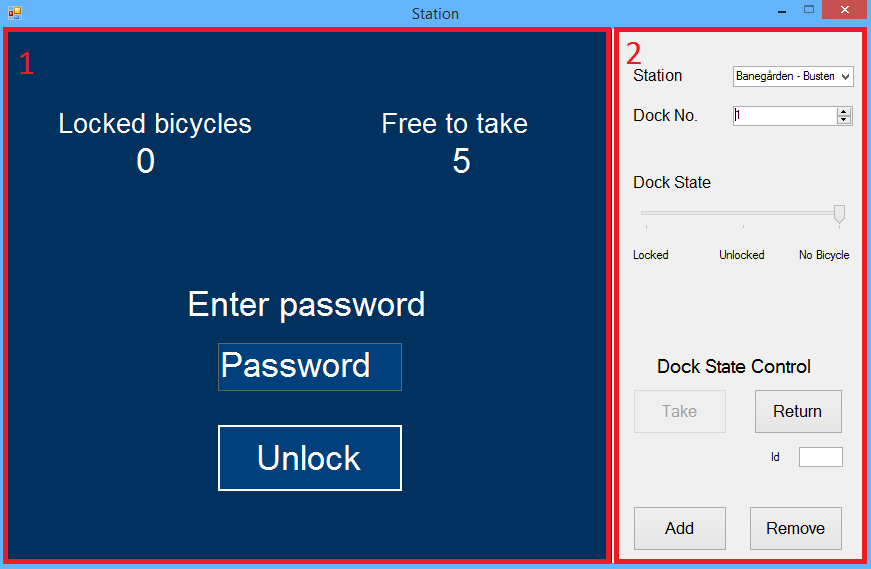
\includegraphics[scale=0.4]{stationsoftware/mainwindow}
	\caption{UI for the station software.}\label{fig:stationMain}
\end{figure}

The station software UI, part 1 in \figref{fig:stationMain}, has been designed to be simple and understandable by users of the system with only the necessary content.
The blue colour was chosen as this is the colour of the bicycles and the \bycykel website.
The station software UI is divided into two pages, the first one can be seen in the figure.
It has a field to input a password for a booking to unlock the booked bicycle.
In addition to this it also displays how many bicycles on the station that are locked and how many that are free to take.
When a valid booking password is input, the station UI changes to the other page, which can be seen in \figref{fig:bicycleUnlock}.
The user is told at which dock the bicycle for him has been unlocked.
There is also a button to quickly return to the main window, which otherwise happens after 10 seconds.

\begin{figure}[h]
	\centering
	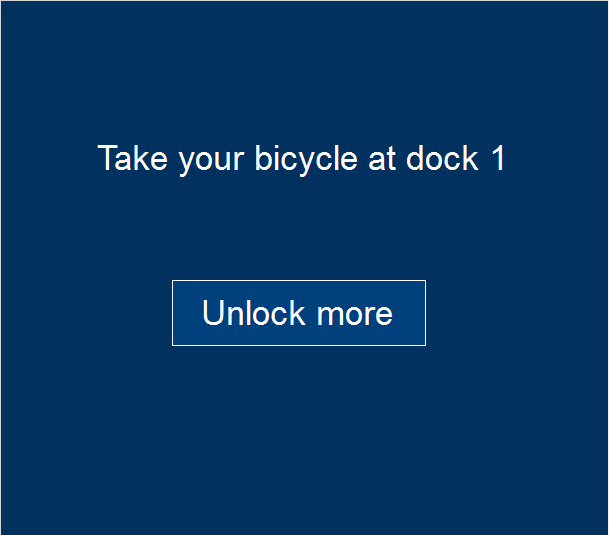
\includegraphics[scale=0.4]{stationsoftware/unlockwindow}
	\caption{UI for unlocked bicycle.}\label{fig:bicycleUnlock}
\end{figure}

\subsection{Station Backend}
The station backend contains three responsibilities as listed below, see \secref{subsec:stationsoftdesfgi}.
\begin{itemize}
	\item A listener that listens for signals from the global database interface called \texttt{WebsiteTo\-StationNotifier}, see \secref{sec:webToStationI}, signalling that a booking has been created or removed.
	\item A lock manager that is responsible for locking a bicycle at a dock when a booking is close to its start time, and unlocking if a booking has expired.
	\item Communication with the global database through a SOAP service interface described in \secref{sec:stationToWebI}.
\end{itemize}

In the following each of these three responsibilities are described further.

\subsubsection{Listener}\label{subsubsec:listener}
The listener is made as a TCP Listener based on code found on Microsofts Developer Network \citep{misc:TcpListenerSource}. 
The listener listens for messages, which is done on port 10000, reporting changes in bookings, either addition or removal of one. 
The messages are JSON encoded strings of different forms depending on the content, two such examples can be seen in \lstref{lst:JsonUnbooking} and \lstref{lst:JsonBooking}.

\begin{minipage}{\textwidth}
\begin{minipage}{0.45\textwidth}
\begin{lstlisting}[caption = {Example of an unbooking message.}, label = {lst:JsonUnbooking}, language=TeX]
{
 "action":"unbooking",
 "start_station":5,
 "booking_id":2
}
\end{lstlisting}
\end{minipage}
\hspace{0.5cm}
\begin{minipage}{0.45\textwidth}
\begin{lstlisting}[caption = {Example of a booking message.}, label = {lst:JsonBooking}, language=TeX]
{
 "action":"booking",
 "start_station":5,
 "booking_id":2,
 "start_time":1414135298,
 "password":483923
}
\end{lstlisting}
\end{minipage}
\end{minipage}

The information contained in the received message is then used to either remove a booking from the database, or add a booking to the database at the specified station, which action to perform is decided based on the action parameter.

\subsubsection{SOAP Service}
%-communication with global DB
The SOAP Service is used to report changes in the local data of the station to the global database, which is implemented in the \texttt{StationToDBRegister} interface, see \secref{sec:stationToWebI}.
The methods in use along with at description of when they are used is listed below.

\begin{description}[style=nextline]
\item[BicycleWithBookingUnlocked] Used when a booking has been used by the user and when a booking has not yet been used but has expired.
\item[BicycleTaken] Used when a bicycle has been taken at a dock possible by means of a booking.
\item[BicycleReturnedToDockAtStation] Used when a bicycle has been returned to a dock.
\item[SyncDockStatus] Used when a dock has been added or removed from a station. It synchronises the status of the docks at that station.
\end{description}

At the start-up or reboot of a station all bookings are synchronised, in order to get updated information for that station, where all bookings are first removed from the station database, and then all bookings are requested from the global database through the interface, using the method \texttt{GetAllBookingsForStation}.
This is done in order to have up to date information and catch bookings performed while the station was offline.

With the communication between the station software and the global database, there is a risk of losing data during the communication or not having a connection at all.
However, this connection loss is taken care of by starting threads that attempt to send the data to the global database every second.
This do give another problem which is when the threads are executed, which does matter because if a bicycle is returned and taken shortly after, the threads can be executed in a different order which makes the system believe that the bicycle is at the station. 
In order to solve this, a queue of function calls are made, so that the function calls are called in the right order, and thereby making this part of the program thread safe.
In other words, the function calls are serialised.
\subsubsection{Lock Manager}
The \texttt{LockManager} runs in its own thread, with the sole responsibility of locking and unlocking docks based on booking start times. 
Currently the time constraints is set to locking a bicycle to a dock one hour before booking start time, and unlocking again one hour after start time, see \secref{subsec:lockingcons}. 
As this functionality requires constant monitoring, the function is run in an infinite thread, however, since we do not want to waste our processor time by executing this constantly, it sleeps for a short period of time after each iteration.

The loop starts out by finding all the expired bookings, removing the lock they had on a bicycle, telling the global database that the bookings have expired, and removing the bookings from the station database.
The loop then finds all bookings that start within the next hour and locks a bicycle for each booking not locked in the last iteration of the loop, if possible. 
It is important to note that if more than one booking start at the same time, the order of docks being locked is given by when the booking was created. 

At the end of the execution of the loop the UI is updated to reflect any changes performed to the database.

\subsection{Simulation of Hardware}
The part of the UI representing the simulated hardware is the second part seen in \figref{fig:stationMain}.
The simulated hardware represents what would normally be observed at the physical station.
We simulate the ID chips on the bicycles and the lock on the dock.
The ID chips are simulated when they would normally have been read at the docks, which is when the bicycles are returned to it after use.
In this case, when a bicycle is returned, we find a random ID from among those not currently in a dock, and selects this as the ID returned.
Random ID is sufficient at this time, as we have no way of predicting where a bicycle in use would be returned to.
Alternatively a bicycle ID can be specified from the GUI, giving more control for illustration purposes.
But for a real station, this can be performed with an RFID chip.
The lock is simulated by a boolean representation, stating if it is locked or not.

In the simulation part of the UI, there is a dropdown list where it is possible to select which station a user is standing at, along with a numeric selector allowing selection of a specific dock at the current station.
In addition, there is also a slide bar showing the state of the selected dock.
The possible states being locked, unlocked, and no bicycle.
At the bottom of the UI there are four buttons that simulate the user actions of returning and removing a bicycle, a field giving the option of specifying which bicycle is returned, and buttons to add and remove docks at the selected station.

For the addition and removal of docks it is handled station-side and not centrally, because otherwise it would require the administrator to add the dock to the system on the website and it could create situations where the administrator adds a dock that does not exist at the station.  
This is of course a design choice that could work in either direction, but due to the reasons given station-side seemed more natural.